%%%%%%%%%%%%%%%%%%%%%%%%%%%%%%%%%%%%%%%%%%%%%%%%%%%%%%%%%%%%%%%%%%%%%%%%%
% Template for a revtex article
%%%%%%%%%%%%%%%%%%%%%%%%%%%%%%%%%%%%%%%%%%%%%%%%%%%%%%%%%%%%%%%%%%%%%%%%%
\documentclass[rmp]{revtex4}
%%%%%%%%%%%%%%%%%%%%%%%%%%%%%%%%%%%%%%%%%%%%%%%%%%%%%%%%%%%%%%%%%%%%%%%%%
\usepackage[english]{babel}
\usepackage[utf8x]{inputenc}
\usepackage{amsmath,amsfonts,amssymb,eucal,eurosym,textcomp}
\usepackage{color}
\usepackage{graphicx}
\usepackage[caption=false]{subfig}
\usepackage{natbib}
\usepackage{pslatex}
\usepackage[colorlinks,linkcolor=red,citecolor=red]{hyperref}
%%%%%%%%%%%%%%%%%%%%%%%%%%%%%%%%%%%%%%%%%%%%%%%%%%%%%%%%%%%%%%%%%%%%%%%%%
\graphicspath{{./figures/}}
%%%%%%%%%%%%%%%%%%%%%%%%%%%%%%%%%%%%%%%%%%%%%%%%%%%%%%%%%%%%%%%%%%%%%%%%%
\newcommand{\comment}[1]{{\color{red}#1}}
%%%%%%%%%%%%%%%%%%%%%%%%%%%%%%%%%%%%%%%%%%%%%%%%%%%%%%%%%%%%%%%%%%%%%%%%%
\renewcommand{\thesubfigure}{\Alph{subfigure}}
\newcommand{\Author}{Fabio~Zanini* and Richard~A.~Neher*}
\newcommand{\Title}{Deleterious synonymous mutations hitchhike to high frequency in HIV \env~evolution}
\newcommand{\Affiliation}{Max Planck Institute for Developmental Biology, 72076 T\"ubingen, Germany}
%%%%%%%%%%%%%%%%%%%%%%%%%%%%%%%%%%%%%%%%%%%%%%%%%%%%%%%%%%%%%%%%%%%%%%%%%
\begin{document}
%%%%%%%%%%%%%%%%%%%%%%%%%%%%%%%%%%%%%%%%%%%%%%%%%%%%%%%%%%%%%%%%%%%%%%%%%
\title{\Title}
\author{\Author}
\affiliation{\textsf{*}\Affiliation}
\date{\today}
\maketitle
%%%%%%%%%%%%%%%%%%%%%%%%%%%%%%%%%%%%%%%%%%%%%%%%%%%%%%%%%%%%%%%%%%%%%%%%%
\tableofcontents

%%%%%%%%%%%%%%%%%%%%%%%%%%%%%%%%%%%%%%%%%%%%%%%%%%%%%%%%%%%%%%%%%%%%%%%%%
\section{Selection of the patient data}
%%%%%%%%%%%%%%%%%%%%%%%%%%%%%%%%%%%%%%%%%%%%%%%%%%%%%%%%%%%%%%%%%%%%%%%%%
\begin{figure}[ht]
\begin{center}
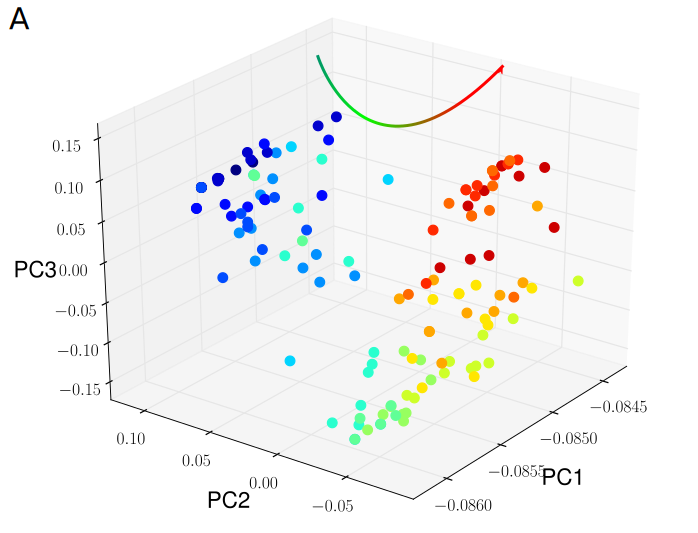
\includegraphics[width=0.35\linewidth]{Shankarappa_PCA_p1}
\includegraphics[width=0.35\linewidth]{Shankarappa_allele_freqs_trajectories_nonsyn_p1}
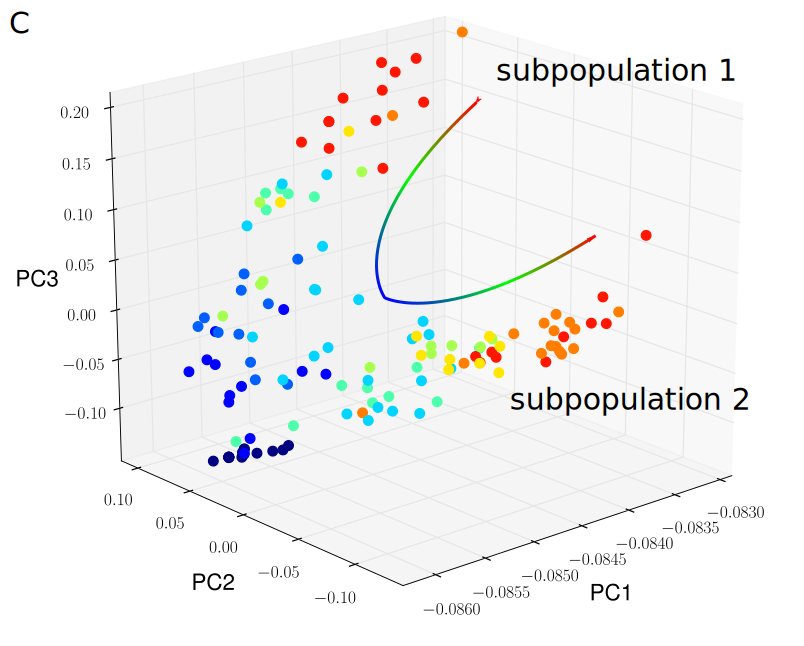
\includegraphics[width=0.35\linewidth]{Shankarappa_PCA_p7}
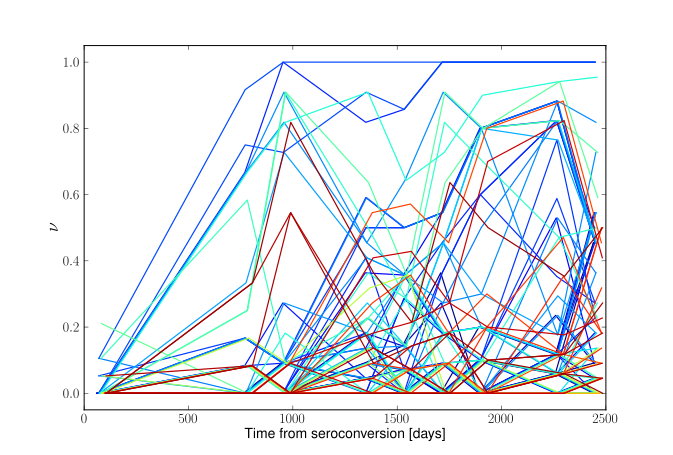
\includegraphics[width=0.35\linewidth]{Shankarappa_allele_freqs_trajectories_nonsyn_p7}
\caption{Panel A) PCA of all sequences from patient p1 (colors indicate time from seroconversion,
from blue to red). Panel B) Allele frequency trajectories for nonsynonymous
changes in the same patient. Panels C and D) show analogous plots for data from
patient p7. Samples after day 1000 split into two clusters in the PCA and no
mutations that arise after day 1000 fix, presumably because they are restricted
to one subpopulation. All patients like p7 (p4, p7, p8, p9 from ref.~\citealp{shankarappa_consistent_1999} and
ACH19542 and ACH19768 from ref.~\citealp{bunnik_autologous_2008}) were excluded
from our analysis.}
\label{fig:aftp}
\end{center}
\end{figure}

%%%%%%%%%%%%%%%%%%%%%%%%%%%%%%%%%%%%%%%%%%%%%%%%%%%%%%%%%%%%%%%%%%%%%%%%%
\section{Synonymous diversity across the HIV genome}
%%%%%%%%%%%%%%%%%%%%%%%%%%%%%%%%%%%%%%%%%%%%%%%%%%%%%%%%%%%%%%%%%%%%%%%%%
\begin{figure}[h]
\begin{center}
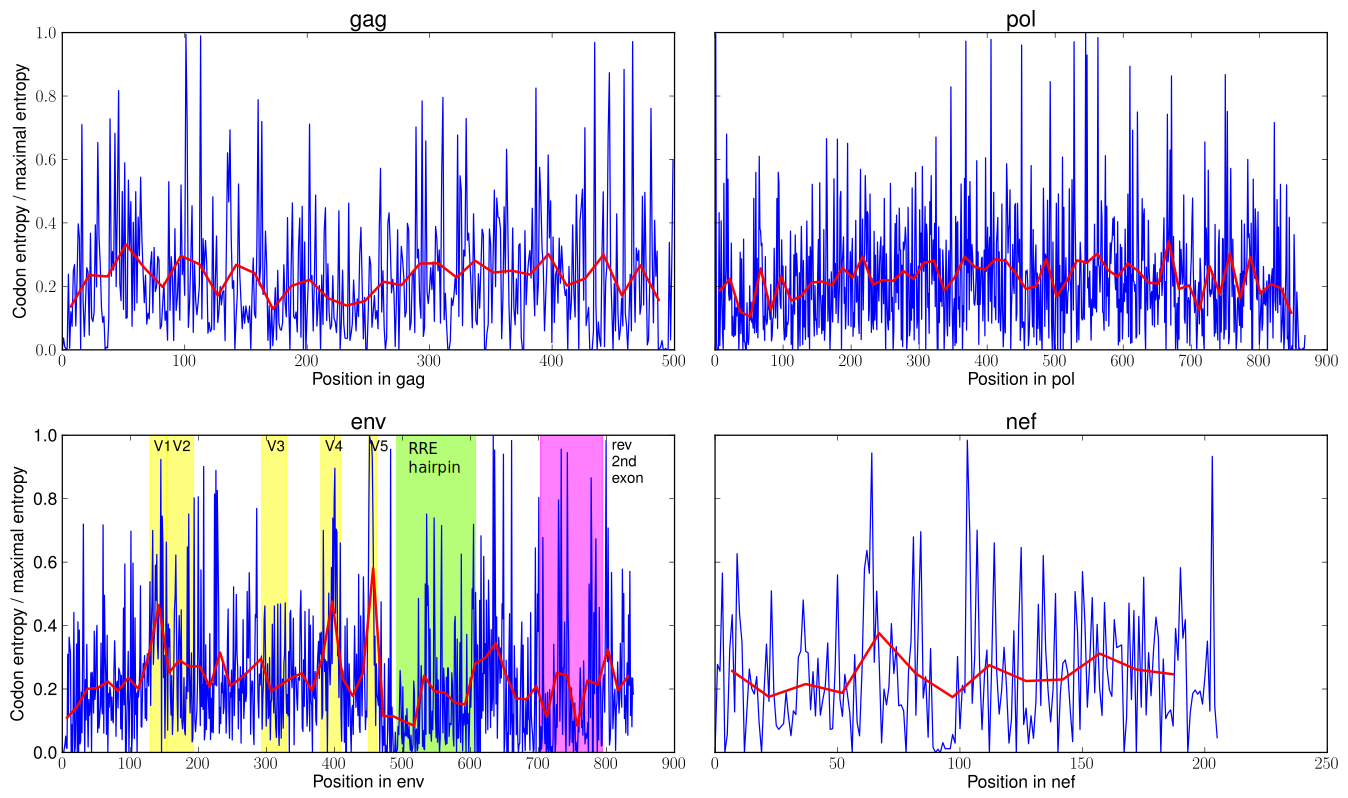
\includegraphics[width=\linewidth]{conservation_codons_genome}
\caption{Synonymous diversity across the HIV genome, as quantified by the
normalized codon entropy. The synonymous diversity peaks at the variable
regions in {\it env} and is reduced in regions under purifying selection (RRE
hairpin, second {\it tat}/{\it rev} exons). Since the variable regions are under
positive selection at the protein level, synonymous hitchhiking is stronger
there, and even deleterious synonymous mutations can be brought to high
frequency. This gives to our signal in the fixation probability, Figs. 2A and
2B of the main text.
The normalized codon entropy is calculated as follows (see the script
for the full algorithm): (i) from a subtype B multiple sequence alignment
(MSA) from the LANL website (filtered sequences only, version 2011)~\cite{LANL2012},
we calculate the consensus amino acid at each position in the HIV genome; (ii) we count
how often each codon coding for the consensus amino acid appears in the MSA;
(iii) at each amino acid position, we divide by the number of sequences in the
MSA that had the consensus amino acid at that position, obtaining {\it codon
frequencies} $\nu_c$; (iv) we calculate the codon entropy from each position as:
$S := - \sum_{c \in \Sigma} \nu_c \log \nu_c$, where $\Sigma$ is the codon
alphabet for that particular amino acid; (v) we divide by the maximal codon entropy of
that amino acid (e.g. $\log 2$ for twofold degenerate codons).
All parts of {\it env} that are part of a different gene (signaling peptide,
second {\it rev} exon) have been excluded from our main analysis, to avoid
contamination about synonymity.}
\label{fig:syndiv_genome}
\end{center}
\end{figure}

%%%%%%%%%%%%%%%%%%%%%%%%%%%%%%%%%%%%%%%%%%%%%%%%%%%%%%%%%%%%%%%%%%%%%%%%%
\section{Nonsynonymous changes outside of variable regions are deleterious}
%%%%%%%%%%%%%%%%%%%%%%%%%%%%%%%%%%%%%%%%%%%%%%%%%%%%%%%%%%%%%%%%%%%%%%%%%
\begin{figure}[h]
\begin{center}
\includegraphics[width=0.4\linewidth]{synmut_conservation_4fold_synnonsyn}
\caption{Cumulative distribution of synonymous and nonsynonymous diversity in
{\it gag} in the LANL reference panel (filtered
sequences only, version 2011)~\cite{LANL2012}. Sites such that the consensus codon
has three synonymous and six nonsynonymous single mutants were used, and the number of observed mutants
of a certain type over the number of possible mutants is plotted. Nonsynonymous
changes are observed less often, {\it ergo} are more conserved, than
synonymous changes. It can be therefore assumed, as mentioned in the main text,
that non-escape nonsynonymous changes involve a large fitness cost.}
\label{fig:synnonsyncons}
\end{center}
\end{figure}

%%%%%%%%%%%%%%%%%%%%%%%%%%%%%%%%%%%%%%%%%%%%%%%%%%%%%%%%%%%%%%%%%%%%%%%%%
\section{Alternative models for suppression of nonsynonymous mutations}
%%%%%%%%%%%%%%%%%%%%%%%%%%%%%%%%%%%%%%%%%%%%%%%%%%%%%%%%%%%%%%%%%%%%%%%%%
\begin{figure}[h]
\begin{center}
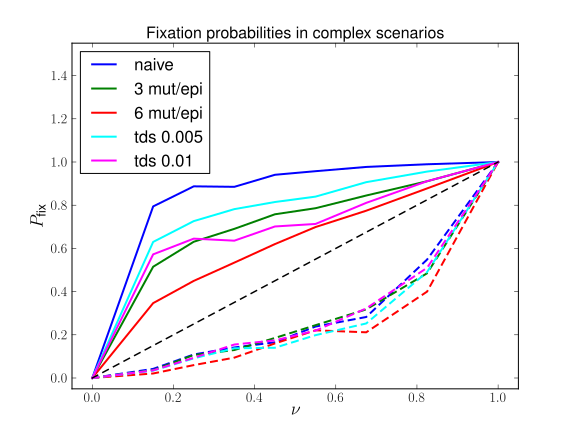
\includegraphics[width=0.5\linewidth]{simulations_graduallyepitopesandtimeselec}
\caption{Time-dependent selection (the escape mutant is recognized after some
months from its appearance) and competition between escape mutations in the same
epitope both reduce fixation of nonsynonymous mutations. A ``na\"ive'' computer
simulation shows a depression in synonymous fixation probability, as observed in
patients, but the nonsynonymous fixation probability is much higher than the
(neutral) diagonal: a nonsynonymous mutation that reaches a frequency around
0.2 is already very likely to fix. In data from infected patients, however,
nonsynonymous mutations show a neutral-like curve,
$P_\text{fix}(\nu) \approx \nu$. In the other curves, we show that the
nonsynonymous fixation probability can be reduced by either time-dependent
selection or competition between equivalent escapes, without affecting much the
synonymous fixation probability itself.
In the curves denoted with ``tds'' (time-dependent selection), the fitness advantage of
an escape mutaition can vanish at each time point with a probability density
\[ P_\text{recognized}(t) = c \cdot \nu(t), \]
where $c$ is a constant coefficient shown in the legend that encodes the overall
efficiency of the host immune system, and $\nu(t)$ is the frequency of the
escape allele at time $t$.
In the curves denoted with ``mut/epi'' we test the
competition scenario instead, with 3 or 6 escape mutations within the same
epitope of length 9 nucleotides. The fitness landscape of each such epitope
include negative epistatic terms, so that the joint presence of more than one
escape mutation is not any more beneficial for the virus than a single mutation.
In this latter scenario, many escape mutations start to sweep on different
backgrounds within the viral population, but eventually compete and only one of
them if fixed.}
\label{fig:tds_wec}
\end{center}
\end{figure}
%%%%%%%%%%%%%%%%%%%%%%%%%%%%%%%%%%%%%%%%%%%%%%%%%%%%%%%%%%%%%%%%%%%%%%%%%
\bibliographystyle{natbib}
\bibliography{bib}
%%%%%%%%%%%%%%%%%%%%%%%%%%%%%%%%%%%%%%%%%%%%%%%%%%%%%%%%%%%%%%%%%%%%%%%%%
\end{document}
%%%%%%%%%%%%%%%%%%%%%%%%%%%%%%%%%%%%%%%%%%%%%%%%%%%%%%%%%%%%%%%%%%%%%%%%%

